% Dit werk is gelicenseerd onder de licentie Creative Commons Naamsvermelding-GelijkDelen 4.0 Internationaal. Ga naar http://creativecommons.org/licenses/by-sa/4.0/ om een kopie van de licentie te kunnen lezen.
\documentclass[t]{beamer}

\usepackage{amsmath,amsthm}             % Uitgebreide wiskundige mogelijkheden
\usepackage{xcolor}						% Om kleuren te gebruiken

%%%%%%%%%%%%%%%%%%%%%%%%%%%%%%%%%%%%%%%%%%%%%%%%%%%%%%%%%%%%
% Nieuwe commandos
%%%%%%%%%%%%%%%%%%%%%%%%%%%%%%%%%%%%%%%%%%%%%%%%%%%%%%%%%%%%

% De differentiaal operator
\newcommand{\diff}{\ensuremath{\mathrm{d}}}
\newcommand{\subsdiff}{\ensuremath{\mathrm{D}}}
\newcommand{\vardiff}{\ensuremath{\mathrm{\delta}}}

% Super en subscript
\newcommand{\supsc}[1]{\ensuremath{^{\text{#1}}}}   % Superscript in tekst
\newcommand{\subsc}[1]{\ensuremath{_{\text{#1}}}}   % Subscript in tekst

% Vectoren en matrices
\newcommand{\vt}[1]{\ensuremath{\boldsymbol{#1}}} % vector in juiste lettertype
\newcommand{\mx}[1]{\ensuremath{\mathsf{#1}}}	  % matrix in juiste lettertype

% Nieuw commando om iets te benadrukken en tegelijkertijd in de index te steken.
\newcommand{\begrip}[1]{\index{#1}\textbf{#1}\xspace}

% Graden celcius
\newcommand{\degC}{\ensuremath{^\circ \mathrm{C}}}
% graden
\renewcommand{\deg}{\ensuremath{^\circ}}

% unit
\newcommand{\unit}[1]{\ensuremath{\mathrm {#1}}}


% underlinered
\newcommand{\underlinered}[1]{\color{red}\underline{{\color{black}#1}}\color{black}}
%%%%%%%%%%%%%%%%%%%%%%%%%%%%%%
% Packages
%%%%%%%%%%%%%%%%%%%%%%%%%%%%%%

%\usepackage{geometry}              	% 
\usepackage[dutch]{babel}               % Voor nederlandstalige hyphenatie (woordsplitsing)
\uselanguage{dutch}
\languagepath{dutch}
\usepackage{amsmath,amsthm}             % Uitgebreide wiskundige mogelijkheden
\usepackage{url}                        % Om url's te verwerken
\usepackage{graphicx,subfigure}         % Om figuren te kunnen verwerken
\usepackage[utf8]{inputenc}             % Om niet ascii karakters rechtstreeks te kunnen typen
\usepackage[section]{placeins}			% Om ervoor te zorgen dat floats binnen dezelfde section blijven
\usepackage{multicol}
\usepackage[absolute,overlay]{textpos}

%%%%%%%%%%%%%%%%%%%%%%%%%%%%%%
% Layout
%%%%%%%%%%%%%%%%%%%%%%%%%%%%%%
\usetheme{Frankfurt}
\usefonttheme[onlymath]{serif}
\AtBeginSection[]
{
  \begin{frame}
    \frametitle{Inhoud}
    \tableofcontents[currentsection]
  \end{frame}
}

\setbeamertemplate{navigation symbols}{}
\setbeamertemplate{footline}[page number]

%%%%%%%%%%%%%%%%%%%%%%%%%%%%%%
% Title
%%%%%%%%%%%%%%%%%%%%%%%%%%%%%%
\title{Fluïdummechanica}
\author{Brecht Baeten\inst{1}}
\institute{
	\inst{1}%
  		KU Leuven, Technologie campus Diepenbeek,\\ e-mail: brecht.baeten@kuleuven.be
}
\date{\today}
%%%%%%%%%%%%%%%%%%%%%%%%%%%%%%
% Omgevingen
%%%%%%%%%%%%%%%%%%%%%%%%%%%%%%


\subtitle{Inleiding}

\begin{document}
	\frame{\titlepage}
	\begin{frame}
		\frametitle{Inleidende voorbeelden}
		\center
    	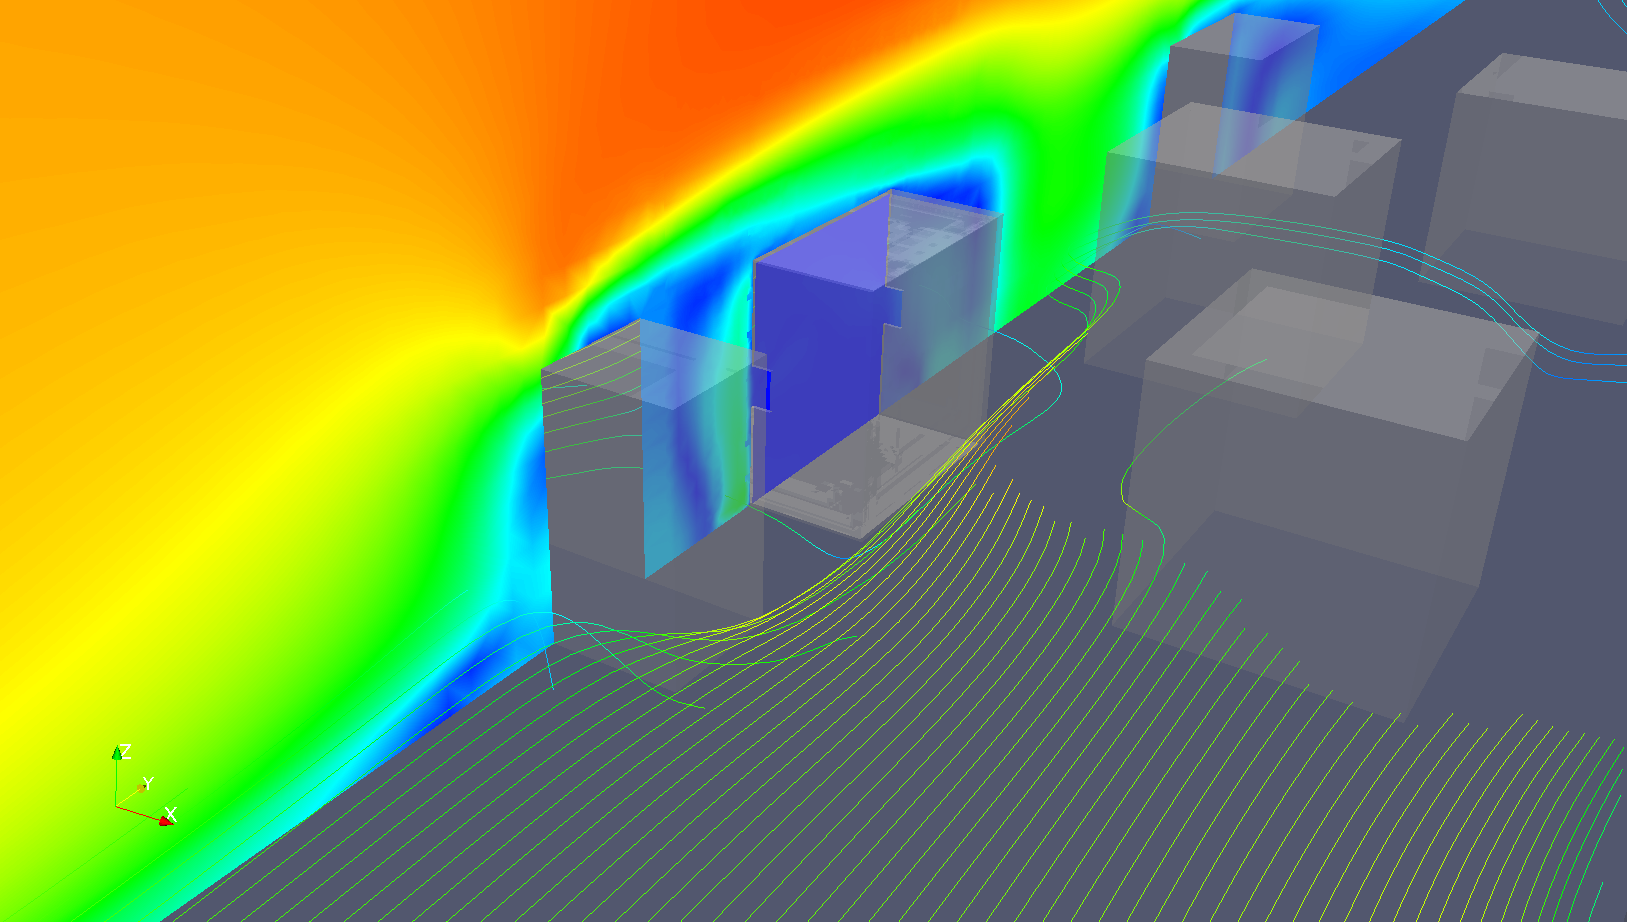
\includegraphics[height=0.7\textheight]{../fig/inleiding/building_neighbourhood_cfd}\\
		\footnotesize{Bron: http://www.refresh-project.org.uk/}
  	\end{frame}
%%%%%%%%%%%%%%%%%%%%%%%%%%%%%%%%%%%%%%%%%%%%%%%%%%%%%%%%%%%%%%%%%%%%%%%%%%%%%%%%%
	\begin{frame}
		\frametitle{Inleidende voorbeelden}
		\center
    	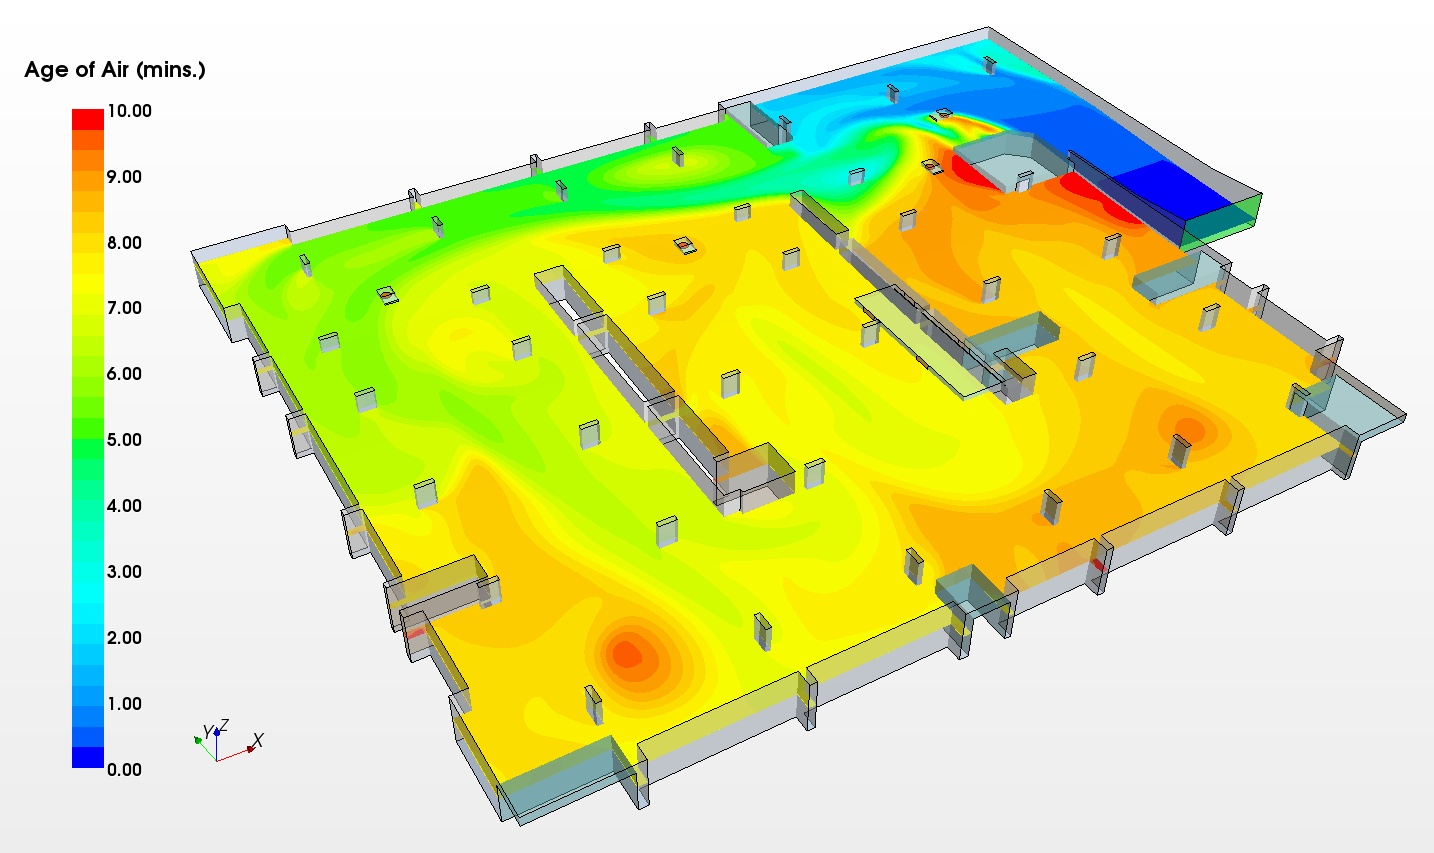
\includegraphics[height=0.7\textheight]{../fig/inleiding/ventilation_cfd}\\
		\footnotesize{Bron: https://www.iesve.com/}
  	\end{frame}
%%%%%%%%%%%%%%%%%%%%%%%%%%%%%%%%%%%%%%%%%%%%%%%%%%%%%%%%%%%%%%%%%%%%%%%%%%%%%%%%%
	\begin{frame}
		\frametitle{Inleidende voorbeelden}
		\center
    	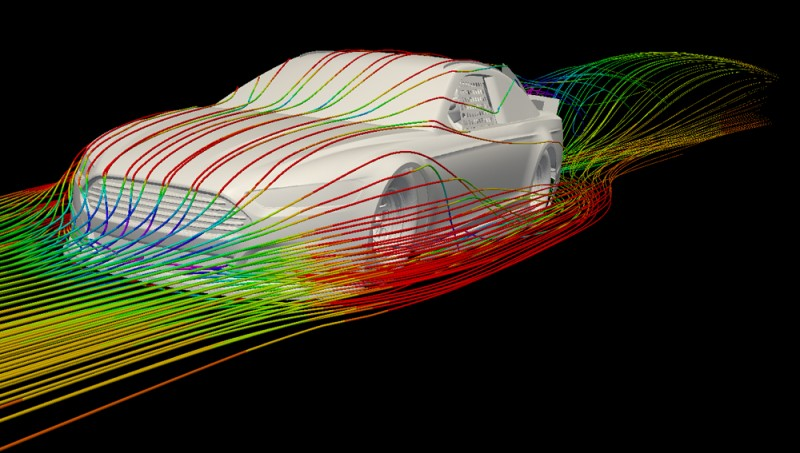
\includegraphics[height=0.7\textheight]{../fig/inleiding/Ford-Fusion-CFD}\\
		\footnotesize{Bron: http://en.wikinoticia.com/}
  	\end{frame}
%%%%%%%%%%%%%%%%%%%%%%%%%%%%%%%%%%%%%%%%%%%%%%%%%%%%%%%%%%%%%%%%%%%%%%%%%%%%%%%%%
	\begin{frame}
		\frametitle{Inleidende voorbeelden}
		\center
    	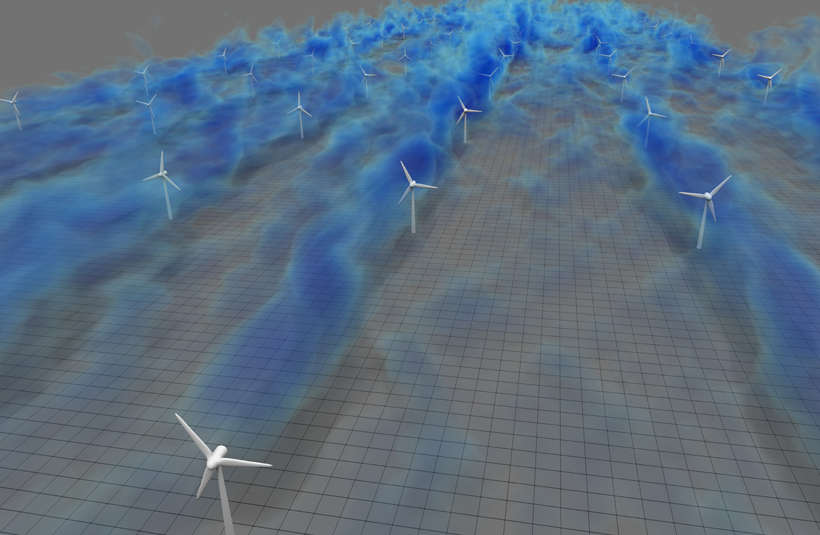
\includegraphics[height=0.7\textheight]{../fig/inleiding/JRSE-Stevens-wind_farms}\\
    	\footnotesize{Bron: https://www.aip.org/}
  	\end{frame}
%%%%%%%%%%%%%%%%%%%%%%%%%%%%%%%%%%%%%%%%%%%%%%%%%%%%%%%%%%%%%%%%%%%%%%%%%%%%%%%%%
	\begin{frame}
		\frametitle{Inleidende voorbeelden}
		\center
    	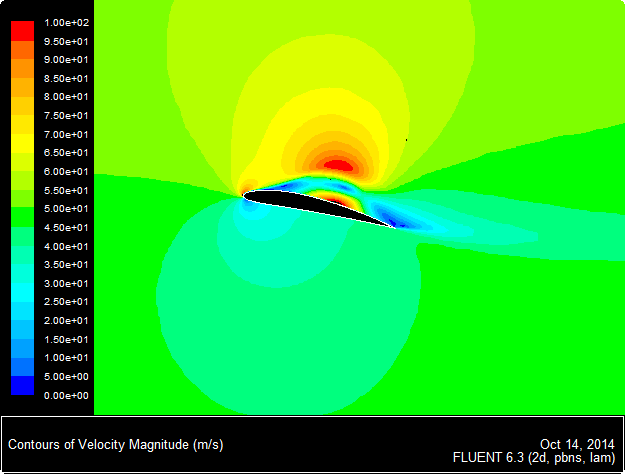
\includegraphics[height=0.7\textheight]{../fig/inleiding/NACA4412_velocity_12deg}\\
  	\end{frame}
%%%%%%%%%%%%%%%%%%%%%%%%%%%%%%%%%%%%%%%%%%%%%%%%%%%%%%%%%%%%%%%%%%%%%%%%%%%%%%%%%
	\begin{frame}
		\frametitle{Inleidende voorbeelden}
		\center
    	\includegraphics[height=0.7\textheight]{../fig/inleiding/pipingnetwork}\\
    	\footnotesize{Bron: http://blogs.intergraph.com/getsmart/}
  	\end{frame}
%%%%%%%%%%%%%%%%%%%%%%%%%%%%%%%%%%%%%%%%%%%%%%%%%%%%%%%%%%%%%%%%%%%%%%%%%%%%%%%%%
	\begin{frame}
		\frametitle{Project}
		\center
    	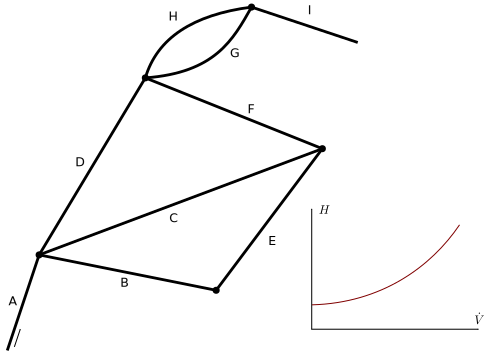
\includegraphics[height=0.8\textheight]{../fig/inleiding/project_leigingkarakteristiek}\\
  	\end{frame}  	
%%%%%%%%%%%%%%%%%%%%%%%%%%%%%%%%%%%%%%%%%%%%%%%%%%%%%%%%%%%%%%%%%%%%%%%%%%%%%%%%%
	\begin{frame}
		\frametitle{ECTS Fiche}
		\begin{itemize}
			\item Examen (8/20 toepassingen, 8/20 theorie)
			\item Project (4/20)
		\end{itemize}
		\begin{itemize}
			\item EC1: Kennis van belangrijke begrippen
			\item EC2: Verklaren van stromings fenomenen
			\item EC4: Verzamelen en verwerken van informatie voor het Project
			\item EC5: Analyseren van stromingsproblemen
			\item EC6: Maken van gepaste veronderstellingen en vereenvoudigingen voor de oplossing van stromingsproblemen
			\item EC8: Inschatten van grootteordes bij stromingsproblemen
			\item EC9: Schrijven van een technisch projectverslag
			\item EC12: Gebruik van duidelijke notaties, omgaan met onbekende materie		
		\end{itemize}
  	\end{frame}
%%%%%%%%%%%%%%%%%%%%%%%%%%%%%%%%%%%%%%%%%%%%%%%%%%%%%%%%%%%%%%%%%%%%%%%%%%%%%%%%%
\end{document}